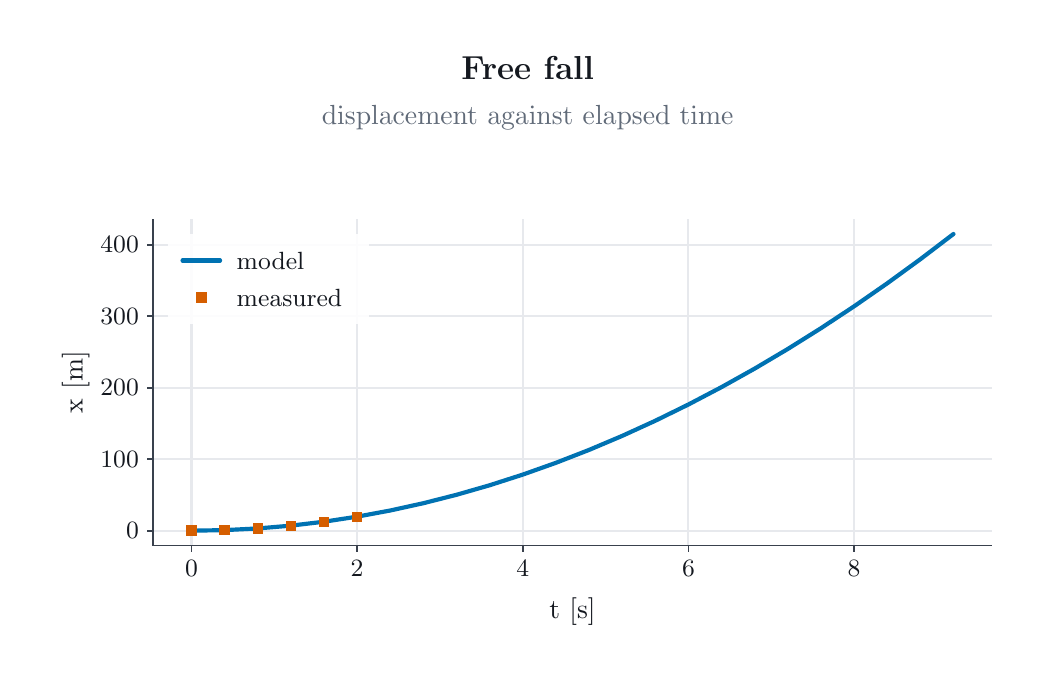
\begin{tikzpicture}[every node/.style={inner sep=0bp,outer sep=0bp}]
  \definecolor{qcA}{rgb}{1,1,1}
  \definecolor{qcB}{rgb}{0.078431,0.094118,0.121569}
  \definecolor{qcC}{rgb}{0.376471,0.415686,0.470588}
  \definecolor{qcD}{rgb}{0.905882,0.913725,0.929412}
  \definecolor{qcE}{rgb}{0,0.447059,0.698039}
  \def\mareymarkF#1#2{\path[fill,shift={(#1,#2)}] (-1.875bp,-1.875bp) rectangle (1.875bp,1.875bp);}
  \definecolor{qcG}{rgb}{0.835294,0.368627,0}
  \definecolor{qcH}{rgb}{0.223529,0.254902,0.301961}
  \useasboundingbox (0bp,0bp) rectangle (360bp,225bp);
  % marey-key: figure
  \path[fill=qcA] (0bp,0bp) -- (360bp,0bp) -- (360bp,225bp) -- (0bp,225bp) -- cycle;
  % marey-role: annotation -- Free fall
  \node[anchor=north,text=qcB,font=\bfseries\fontsize{13}{15.6}\selectfont] at (180bp,214.5bp) {Free fall};
  \node[anchor=north,text=qcC,font=\fontsize{10}{12}\selectfont] at (180bp,197.225bp) {displacement against elapsed time};
  % marey-role: other:panel -- panel
  % marey-data: row = 0
  % marey-data: col = 0
  % marey-data: layers = 2
  % marey-data: x-tick-rule = all
  % marey-data: y-tick-rule = all
  % marey-role: decoration -- gridlines
  % marey-data: lines = 10
  \path[draw=qcD,line width=0.75bp] (58.977bp,38.575bp) -- (58.977bp,156.063bp) (118.609bp,38.575bp) -- (118.609bp,156.063bp) (178.241bp,38.575bp) -- (178.241bp,156.063bp) (237.872bp,38.575bp) -- (237.872bp,156.063bp) (297.504bp,38.575bp) -- (297.504bp,156.063bp) (45.262bp,43.915bp) -- (346.998bp,43.915bp) (45.262bp,69.642bp) -- (346.998bp,69.642bp) (45.262bp,95.369bp) -- (346.998bp,95.369bp) (45.262bp,121.095bp) -- (346.998bp,121.095bp) (45.262bp,146.822bp) -- (346.998bp,146.822bp);
  \begin{scope}
    \clip (45.262bp,38.575bp) -- (346.998bp,38.575bp) -- (346.998bp,156.063bp) -- (45.262bp,156.063bp) -- cycle;
    % marey-role: series -- model
    % marey-data: series = model
    % marey-data: points = 24
    \path[draw=qcE,line width=1.5bp,line cap=round,line join=round] (58.977bp,43.915bp) -- (70.904bp,44.117bp) -- (82.83bp,44.723bp) -- (94.756bp,45.732bp) -- (106.683bp,47.146bp) -- (118.609bp,48.963bp) -- (130.535bp,51.184bp) -- (142.462bp,53.809bp) -- (154.388bp,56.837bp) -- (166.314bp,60.27bp) -- (178.241bp,64.106bp) -- (190.167bp,68.346bp) -- (202.093bp,72.989bp) -- (214.019bp,78.037bp) -- (225.946bp,83.488bp) -- (237.872bp,89.344bp) -- (249.798bp,95.603bp) -- (261.725bp,102.265bp) -- (273.651bp,109.332bp) -- (285.577bp,116.802bp) -- (297.504bp,124.677bp) -- (309.43bp,132.955bp) -- (321.356bp,141.637bp) -- (333.283bp,150.722bp);
    % marey-role: series -- measured
    % marey-data: series = measured
    % marey-data: points = 6
    \begin{scope}[fill=qcG]
      \mareymarkF{58.977bp}{43.915bp}
      \mareymarkF{70.904bp}{44.113bp}
      \mareymarkF{82.83bp}{44.706bp}
      \mareymarkF{94.756bp}{45.694bp}
      \mareymarkF{106.683bp}{47.077bp}
      \mareymarkF{118.609bp}{48.855bp}
    \end{scope}
  \end{scope}
  % marey-role: axis -- t [s]
  % marey-data: side = bottom
  % marey-data: unit = s
  % marey-data: prefix =
  % marey-data: ticks = 5
  % marey-data: tick-rule = all
  \path[draw=qcH,line width=0.675bp] (45.262bp,38.575bp) -- (346.998bp,38.575bp);
  \path[draw=qcH,line width=0.675bp] (58.977bp,38.575bp) -- (58.977bp,36.325bp) (118.609bp,38.575bp) -- (118.609bp,36.325bp) (178.241bp,38.575bp) -- (178.241bp,36.325bp) (237.872bp,38.575bp) -- (237.872bp,36.325bp) (297.504bp,38.575bp) -- (297.504bp,36.325bp);
  \node[anchor=north,text=qcB,font=\fontsize{9}{10.8}\selectfont] at (58.977bp,33.325bp) {0};
  \node[anchor=north,text=qcB,font=\fontsize{9}{10.8}\selectfont] at (118.609bp,33.325bp) {2};
  \node[anchor=north,text=qcB,font=\fontsize{9}{10.8}\selectfont] at (178.241bp,33.325bp) {4};
  \node[anchor=north,text=qcB,font=\fontsize{9}{10.8}\selectfont] at (237.872bp,33.325bp) {6};
  \node[anchor=north,text=qcB,font=\fontsize{9}{10.8}\selectfont] at (297.504bp,33.325bp) {8};
  \node[anchor=north,text=qcB,font=\fontsize{10}{12}\selectfont] at (196.13bp,19.75bp) {t [s]};
  % marey-role: axis -- x [m]
  % marey-data: side = left
  % marey-data: unit = m
  % marey-data: prefix =
  % marey-data: ticks = 5
  % marey-data: tick-rule = all
  \path[draw=qcH,line width=0.675bp] (45.262bp,38.575bp) -- (45.262bp,156.063bp);
  \path[draw=qcH,line width=0.675bp] (45.262bp,43.915bp) -- (43.012bp,43.915bp) (45.262bp,69.642bp) -- (43.012bp,69.642bp) (45.262bp,95.369bp) -- (43.012bp,95.369bp) (45.262bp,121.095bp) -- (43.012bp,121.095bp) (45.262bp,146.822bp) -- (43.012bp,146.822bp);
  \node[anchor=east,text=qcB,font=\fontsize{9}{10.8}\selectfont] at (40.012bp,43.915bp) {0};
  \node[anchor=east,text=qcB,font=\fontsize{9}{10.8}\selectfont] at (40.012bp,69.642bp) {100};
  \node[anchor=east,text=qcB,font=\fontsize{9}{10.8}\selectfont] at (40.012bp,95.369bp) {200};
  \node[anchor=east,text=qcB,font=\fontsize{9}{10.8}\selectfont] at (40.012bp,121.095bp) {300};
  \node[anchor=east,text=qcB,font=\fontsize{9}{10.8}\selectfont] at (40.012bp,146.822bp) {400};
  \node[anchor=base,text=qcB,rotate=90,font=\fontsize{10}{12}\selectfont] at (19.75bp,97.319bp) {x [m]};
  % marey-role: legend -- legend
  % marey-data: entries = 2
  \path[fill=qcA,fill opacity=0.9] (50.512bp,118.238bp) -- (122.749bp,118.238bp) -- (122.749bp,150.813bp) -- (50.512bp,150.813bp) -- cycle;
  % marey-role: other:legend-entry -- model
  % marey-data: series = model
  % marey-data: color = #0072b2
  \path[draw=qcE,line width=1.5bp,line cap=round] (55.762bp,141.169bp) -- (69.262bp,141.169bp);
  \node[anchor=west,text=qcB,font=\fontsize{9.5}{11.4}\selectfont] at (75.262bp,141.169bp) {model};
  % marey-role: other:legend-entry -- measured
  % marey-data: series = measured
  % marey-data: color = #d55e00
  \begin{scope}[fill=qcG]
    \mareymarkF{62.512bp}{127.881bp}
  \end{scope}
  \node[anchor=west,text=qcB,font=\fontsize{9.5}{11.4}\selectfont] at (75.262bp,127.881bp) {measured};
\end{tikzpicture}
